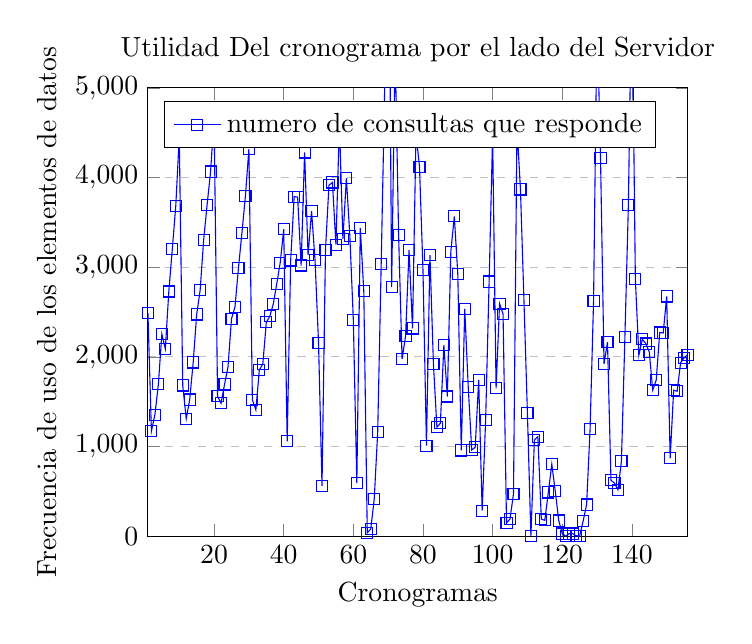
\begin{tikzpicture}
\begin{axis}[
    title={Utilidad Del cronograma por el lado del Servidor},
    xlabel={Cronogramas},
    ylabel={Frecuencia de uso de los elementos de datos},
    xmin=1, xmax=156,
    ymin=0, ymax=5000,
    xtick={},
    ytick={},
    legend pos=north west,
    ymajorgrids=true,
    grid style=dashed,
]

\addplot[
    color=blue,
    mark=square,
    ]
    coordinates {
%UTILIDAD TOTAL
%(cronograma, numero cues que usan al cronograma)
(1,2489)
(2,1172)
(3,1354)
(4,1695)
(5,2254)
(6,2089)
(7,2729)
(8,3202)
(9,3684)
(10,4452)
(11,1681)
(12,1310)
(13,1524)
(14,1938)
(15,2473)
(16,2744)
(17,3302)
(18,3697)
(19,4067)
(20,4671)
(21,1560)
(22,1482)
(23,1692)
(24,1887)
(25,2424)
(26,2557)
(27,2990)
(28,3383)
(29,3794)
(30,4318)
(31,1520)
(32,1408)
(33,1855)
(34,1920)
(35,2385)
(36,2452)
(37,2589)
(38,2816)
(39,3050)
(40,3423)
(41,1057)
(42,3075)
(43,3787)
(44,3782)
(45,3019)
(46,4280)
(47,3134)
(48,3624)
(49,3076)
(50,2159)
(51,562)
(52,3196)
(53,3914)
(54,3945)
(55,3251)
(56,4606)
(57,3315)
(58,3992)
(59,3345)
(60,2412)
(61,591)
(62,3437)
(63,2734)
(64,38)
(65,80)
(66,413)
(67,1166)
(68,3034)
(69,5002)
(70,8214)
(71,2779)
(72,5464)
(73,3358)
(74,1975)
(75,2232)
(76,3190)
(77,2317)
(78,4493)
(79,4119)
(80,2970)
(81,1010)
(82,3136)
(83,1922)
(84,1216)
(85,1259)
(86,2130)
(87,1558)
(88,3173)
(89,3567)
(90,2926)
(91,956)
(92,2534)
(93,1663)
(94,961)
(95,992)
(96,1742)
(97,285)
(98,1300)
(99,2840)
(100,4464)
(101,1649)
(102,2593)
(103,2477)
(104,147)
(105,192)
(106,473)
(107,4572)
(108,3867)
(109,2633)
(110,1370)
(111,0)
(112,1073)
(113,1110)
(114,190)
(115,177)
(116,488)
(117,802)
(118,500)
(119,174)
(120,29)
(121,0)
(122,29)
(123,29)
(124,5)
(125,2)
(126,168)
(127,353)
(128,1197)
(129,2626)
(130,5842)
(131,4217)
(132,1922)
(133,2163)
(134,623)
(135,592)
(136,517)
(137,836)
(138,2220)
(139,3697)
(140,6329)
(141,2866)
(142,2017)
(143,2196)
(144,2148)
(145,2055)
(146,1628)
(147,1744)
(148,2271)
(149,2266)
(150,2674)
(151,868)
(152,1628)
(153,1616)
(154,1935)
(155,1988)
(156,2024)
(157,2357)
(158,2531)
(159,2844)
(160,3456)
(161,1104)
(162,2631)
    };
    \legend{numero de consultas que responde}

\end{axis}
\end{tikzpicture}

